\documentclass[pdflatex,sn-mathphys-num]{sn-jnl}% Math and Physical Sciences Numbered Reference Style

%%%% Standard Packages
\usepackage{graphicx}%
\usepackage{multirow}%
\usepackage{amsmath,amssymb,amsfonts}%
\usepackage{amsthm}%
\usepackage{mathrsfs}%
\usepackage[title]{appendix}%
\usepackage{xcolor}%
\usepackage{textcomp}%
\usepackage{manyfoot}%
\usepackage{booktabs}%
\usepackage{algorithm}%
\usepackage{algorithmicx}%
\usepackage{algpseudocode}%
\usepackage{listings}%

\theoremstyle{thmstyleone}%
\newtheorem{theorem}{Theorem}%
\newtheorem{proposition}[theorem]{Proposition}%

\theoremstyle{thmstyletwo}%
\newtheorem{example}{Example}%
\newtheorem{remark}{Remark}%

\theoremstyle{thmstylethree}%
\newtheorem{definition}{Definition}%

\raggedbottom

\begin{document}

\title[Anomaly Detection on Smart Home Energy Data]{Anomaly Detection on Smart Home Energy Data: A Comparative Machine Learning Study with a Statistical Proxy-Labelling Strategy}

%%=============================================================%%
%% Authors %%
%%=============================================================%%

\author*[1]{\fnm{Xuan Binh} \sur{Nguyen}}\email{author1@example.com}

\author[1]{\fnm{Quang Hung} \sur{Bui Doan}}\email{author2@example.com}
\equalcont{These authors contributed equally to this work.}

\author[1]{\fnm{Quoc Chung} \sur{Le}}\email{author3@example.com}
\equalcont{These authors contributed equally to this work.}

\affil*[1]{\orgdiv{Department of Information Technology}, \orgname{[University Name]}, \orgaddress{\city{Ho Chi Minh City}, \country{Vietnam}}}

%%==================================%%
%% Abstract %%
%%==================================%%

\abstract{Smart home energy systems generate large volumes of high-resolution consumption data, within which abnormal usage periods may signal equipment faults, inefficient operation, or unusual occupant behaviour. A central difficulty in this domain is that publicly available energy datasets rarely contain labelled anomaly events, which prevents the direct use of supervised classification and standard threshold-independent evaluation. This study addresses that difficulty using the publicly available Smart Home Dataset with Weather Information (HomeC), comprising 503{,}910 minute-level observations across 32 attributes. We construct a transparent statistical proxy label by flagging observations whose total household consumption exceeds the mean plus three standard deviations, yielding an anomaly rate of approximately 2.46\%. We deliberately treat this as a proxy rather than ground truth and discuss its limitations explicitly. The labelled data is then framed as a binary classification task. After cleaning, feature construction (55 features) and a stratified train--test split, the minority class is balanced on the training partition only using SMOTE, and five models are compared: Logistic Regression, Random Forest, XGBoost, LightGBM and Isolation Forest. Random Forest achieved the strongest performance (F1 = 0.9343, AUC = 0.9995), while the unsupervised Isolation Forest performed markedly worse (F1 = 0.0818), illustrating the gap between supervised and unsupervised paradigms under proxy supervision. We report the dataset's known timestamp limitation as a constraint on temporal features. The trained pipeline is exported and integrated into an interactive dashboard for single-observation prediction.}

\keywords{anomaly detection, smart home, energy consumption, machine learning, proxy labelling, class imbalance, SMOTE}

\maketitle

%%=============================================================%%
\section{Introduction}\label{sec1}

The increasing deployment of smart home technologies has enabled continuous, fine-grained monitoring of household electricity consumption through connected sensors and smart meters. These systems produce large time-series datasets that can be analysed to improve energy efficiency, reduce operating costs and support automated home management. Within these data streams, abnormal consumption periods may indicate equipment malfunction, energy leakage, inefficient usage, or unusual occupant activity, and detecting them early can help reduce energy costs and extend equipment lifespan \cite{himeur2021}.

Traditional monitoring approaches often rely on manual inspection or fixed predefined thresholds, which struggle to capture complex abnormal patterns in large-scale data. Machine learning offers a more scalable alternative by learning consumption behaviour directly from historical observations \cite{ambat2025}. A persistent obstacle, however, is the scarcity of labelled anomaly events: there is no widely available residential energy dataset with curated ground-truth anomaly labels \cite{ambat2025}. This forces practitioners either toward unsupervised methods or toward constructing proxy labels from statistical criteria.

This work takes the latter route in a deliberately transparent way. Using the publicly available Smart Home Dataset with Weather Information (HomeC), we define a statistical proxy label for abnormal consumption and reformulate the problem as binary classification. This reformulation allows the use of threshold-aware metrics such as the F1-score and the area under the ROC curve (AUC-ROC), and enables a like-for-like comparison of multiple models. We emphasise throughout that the resulting labels are a proxy and not verified ground truth, and we discuss the implications of this choice for the validity of the reported results.

The contributions of this study are: (i) a transparent statistical proxy-labelling procedure grounded in prior energy-domain practice; (ii) a controlled comparison of five models spanning linear, ensemble and unsupervised families on the same data partition; and (iii) an end-to-end pipeline, exported and embedded in an interactive prediction dashboard. We also document a known data-quality limitation of the HomeC dataset that affects the temporal features.

%%=============================================================%%
\section{Research Questions}\label{sec2}

The study is guided by three research questions:

\begin{itemize}
\item \textbf{RQ1.} Which appliance-related and weather-related variables are associated with abnormal energy consumption?
\item \textbf{RQ2.} Which model performs best at detecting abnormal consumption events on this dataset?
\item \textbf{RQ3.} Does weather influence abnormal household energy consumption?
\end{itemize}

%%=============================================================%%
\section{Related Work}\label{sec3}

Anomaly detection in residential energy consumption has been approached through statistical, machine learning and deep learning techniques \cite{himeur2021}. Statistical methods such as the Z-score and the interquartile range (IQR) provide an intuitive and computationally light way to flag deviations from typical consumption, and they are commonly used as baselines, though they can misclassify points in the presence of noisy or inconsistent data \cite{abnormality2024}. Notably, prior work applying statistical and learning-based methods directly to the same HomeC dataset has documented that it contains data-quality issues, including missing values, redundancies, outliers and garbage records \cite{abnormality2024}; we take account of this in our cleaning stage.

A recurring theme in the literature is the absence of labelled ground-truth anomalies in real energy datasets. Ambat and Sahoo note this explicitly and adopt outlier-based techniques to derive anomalies before training predictive models \cite{ambat2025}. Our statistical proxy-labelling strategy is in the same spirit: rather than asserting that a flagged point is a true anomaly, we use a transparent statistical rule to obtain weak labels and are explicit that these are proxies. Ensemble methods such as Random Forest \cite{breiman2001random}, gradient boosting variants \cite{chen2016xgboost,ke2017lightgbm}, and the unsupervised Isolation Forest \cite{liu2008isolation} are widely used in this area, and we evaluate representatives of each.

%%=============================================================%%
\section{Data and Methodology}\label{sec4}

\subsection{Dataset}\label{subsec:data}

The Smart Home Dataset with Weather Information (HomeC), obtained from Kaggle, contains 503{,}910 observations and 32 attributes recorded at minute-level resolution. The attributes fall into three groups: overall energy variables (e.g. \texttt{use [kW]}, \texttt{gen [kW]}), appliance-level consumption (e.g. dishwasher, furnace, fridge, microwave, living room, garage, barn, well), and weather variables (temperature, humidity, visibility, pressure, wind speed, cloud cover, dew point, precipitation probability and intensity).

\subsection{Data cleaning}\label{subsec:clean}

Duplicate columns containing redundant information (\texttt{House overall [kW]} and \texttt{Solar [kW]}) were removed to reduce multicollinearity, and constant columns were dropped. Duplicate-row analysis returned no duplicated observations. Extreme values identified by the IQR method (34{,}211 observations) were retained rather than removed, since in an anomaly-detection context such values may correspond to the very behaviour of interest rather than measurement error.

\subsection{Statistical proxy labelling}\label{subsec:label}

Because the dataset contains no ground-truth anomaly labels, we construct a proxy label from a statistical threshold on total consumption. Let $\mu$ and $\sigma$ denote the mean and standard deviation of \texttt{use [kW]}. An observation is labelled anomalous when its consumption exceeds a $k$-sigma threshold:

\begin{equation}
\text{anomaly}_i =
\begin{cases}
1, & \text{if } \texttt{use [kW]}_i > \mu + k\,\sigma \\
0, & \text{otherwise}
\end{cases}
\label{eq:label}
\end{equation}

We set $k = 3$, which yields an anomaly rate of approximately 2.46\%, within the 1--5\% range typically expected for rare-event detection. This rule follows established statistical practice in the energy-anomaly literature, where deviation-from-typical-consumption criteria such as Z-score thresholds are standard baselines \cite{abnormality2024,ambat2025}.

\begin{remark}
The labels produced by Eq.~\eqref{eq:label} are a \emph{proxy}, not verified ground truth. They encode the assumption that statistically extreme total consumption corresponds to a genuine anomaly, which need not always hold (for example, a legitimate but rare high-demand period). All results in this paper should be read as performance against this proxy definition rather than against externally validated anomalies. We consider this transparency preferable to presenting the proxy as if it were ground truth.
\end{remark}

\subsection{Feature construction}\label{subsec:feat}

Four temporal features (\texttt{hour}, \texttt{dayofweek}, \texttt{month}, \texttt{is\_weekend}) were derived from the timestamp. The two textual weather fields (\texttt{icon}, \texttt{summary}) were one-hot encoded. The column \texttt{use [kW]} was excluded from the feature set because it is used to define the label; retaining it would constitute direct target leakage. The final feature matrix contained 55 columns.

\begin{remark}[Data-quality limitation]
Inspection of the timestamp field revealed a known issue with this dataset: the parsed \texttt{datetime} column spans only about six days rather than the full year suggested by the dataset description, because the underlying Unix timestamp increments per second rather than per minute. As a consequence, the \texttt{month}, \texttt{dayofweek} and \texttt{is\_weekend} features carry little information, whereas \texttt{hour} remains usable. We report this limitation rather than removing it silently, and treat seasonal conclusions with corresponding caution.
\end{remark}

\subsection{Partitioning and class balancing}\label{subsec:split}

The data was split into training (80\%) and test (20\%) partitions with stratification on the label and a fixed random seed for reproducibility. Standardisation was fitted on the training partition only and applied to the test partition, avoiding information leakage. To address class imbalance, SMOTE \cite{chawla2002} was applied to the training partition only; the test partition retained its natural class distribution so that reported metrics reflect realistic conditions.

\subsection{Models and evaluation}\label{subsec:models}

Five models were trained on the same partition: Logistic Regression, Random Forest \cite{breiman2001random}, XGBoost \cite{chen2016xgboost}, LightGBM \cite{ke2017lightgbm}, and Isolation Forest \cite{liu2008isolation}. The first four are supervised; Isolation Forest is unsupervised and was trained without labels, included to contrast the two paradigms. Following common practice on large datasets, kernel SVM variants were excluded because of their poor scalability to the full data volume \cite{pedregosa2011scikit}.

Given the class imbalance, accuracy is unsuitable as a primary metric: a trivial classifier predicting the majority class would still score highly. We therefore report the F1-score, AUC-ROC, precision and recall. The F1-score is the harmonic mean of precision and recall:

\begin{equation}
\text{F1} = 2 \cdot \frac{\text{Precision} \cdot \text{Recall}}{\text{Precision} + \text{Recall}}.
\label{eq:f1}
\end{equation}

The best-performing supervised model was then tuned with randomised hyperparameter search under stratified cross-validation, and the final pipeline (standardisation plus the chosen model) was exported for deployment.

%%=============================================================%%
\section{Exploratory Data Analysis}\label{sec5}

The exploratory analysis characterises consumption behaviour and motivates the modelling choices.

\begin{figure}[h]
\centering
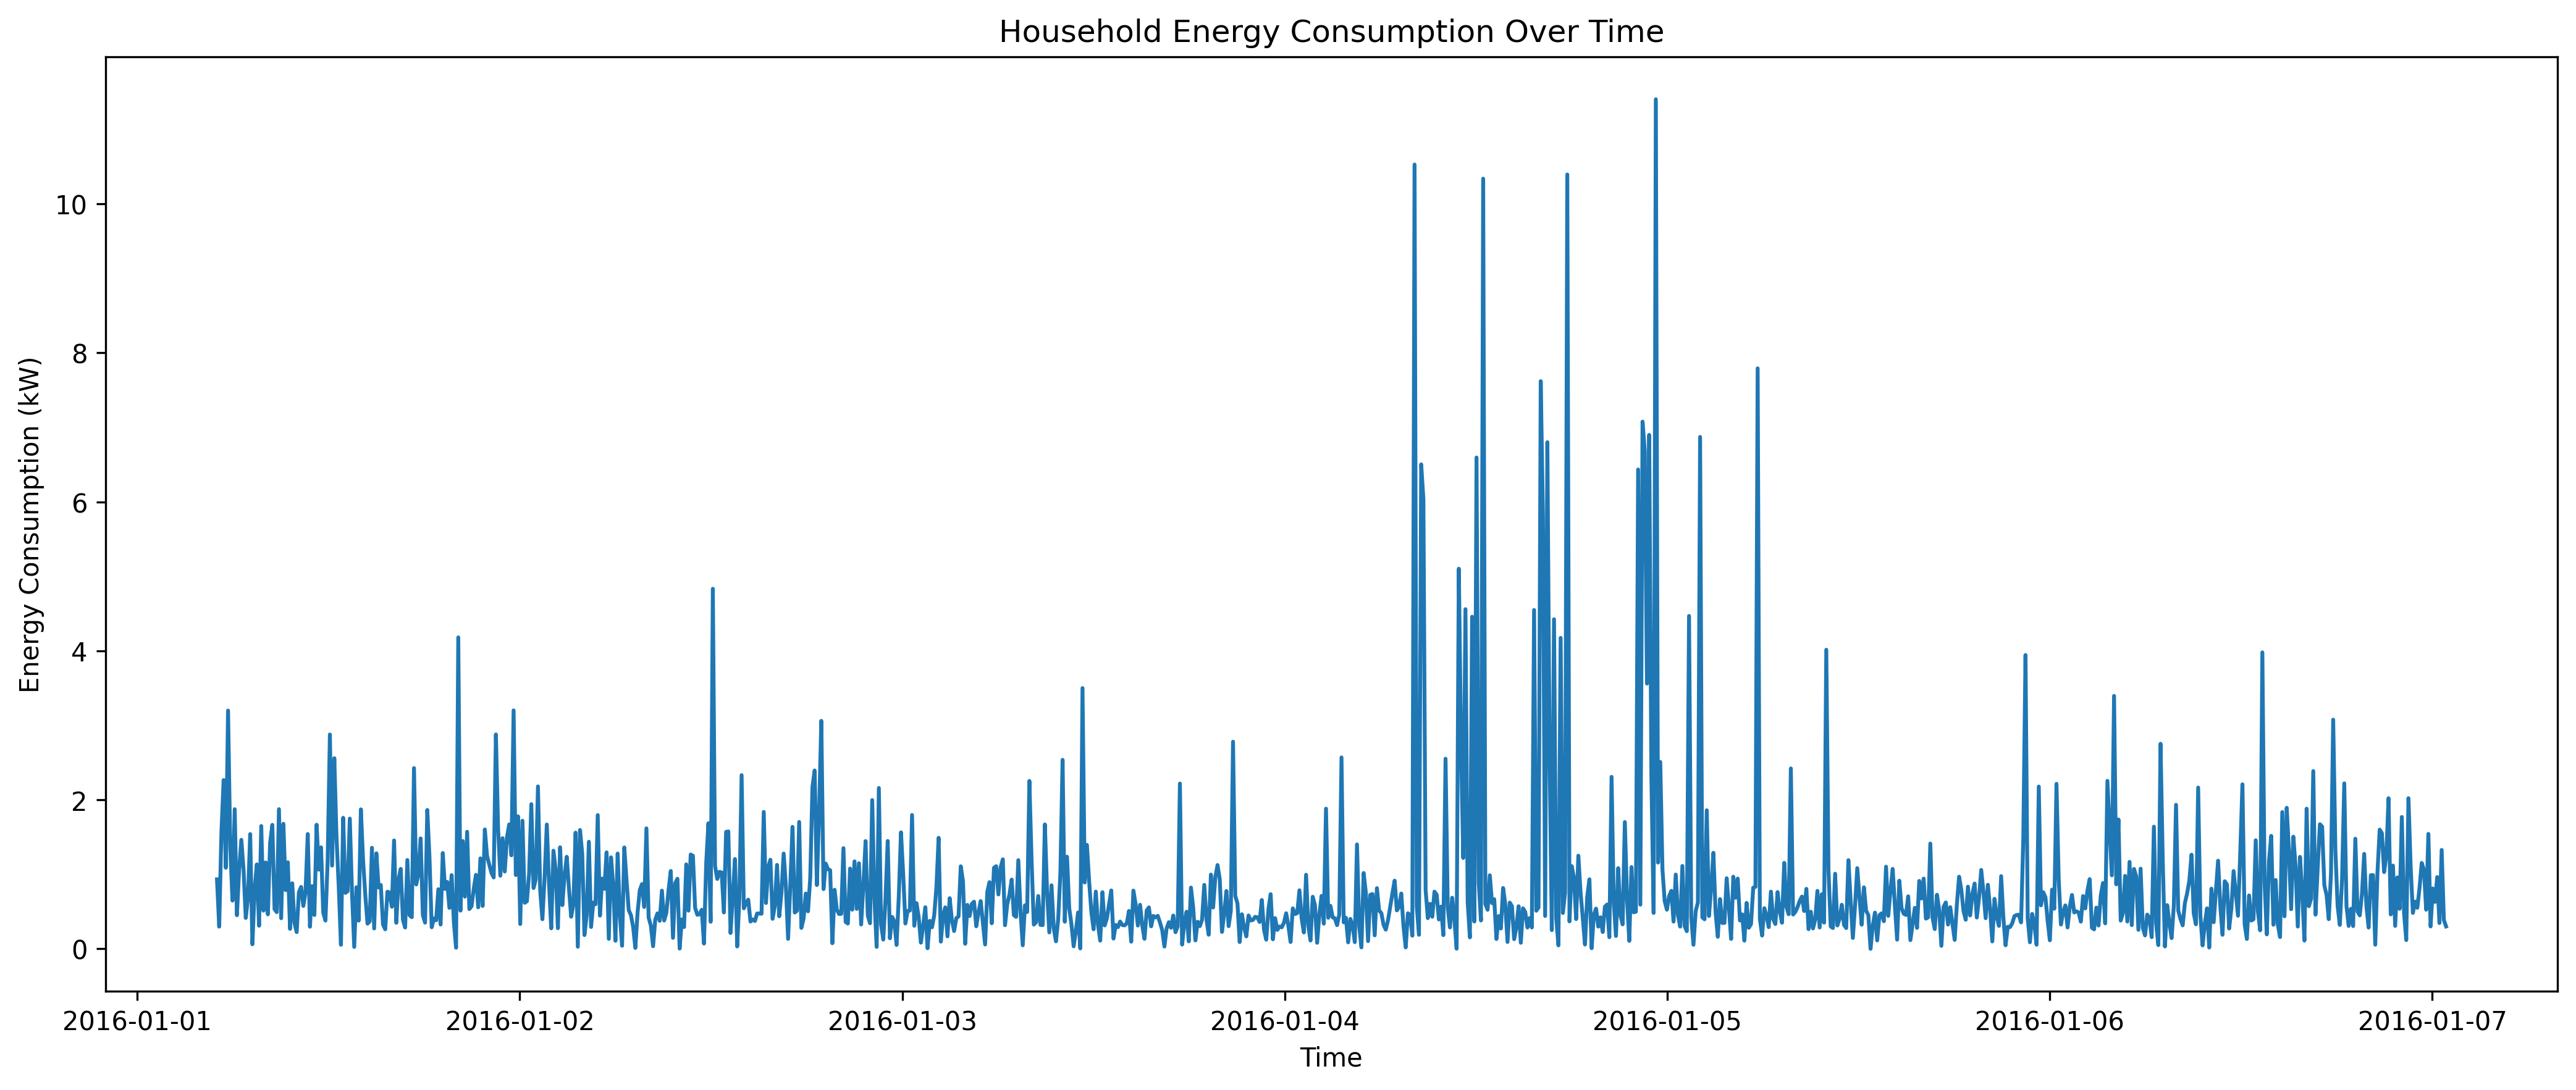
\includegraphics[width=0.95\textwidth]{chart1_timeseries.png}
\caption{Household total energy consumption over the observed period. Pronounced spikes correspond to periods of unusually high usage and represent candidate anomalies.}\label{fig:ts}
\end{figure}

Figure~\ref{fig:ts} shows that consumption fluctuates considerably, with several sharp spikes consistent with abnormal usage events.

\begin{figure}[h]
\centering
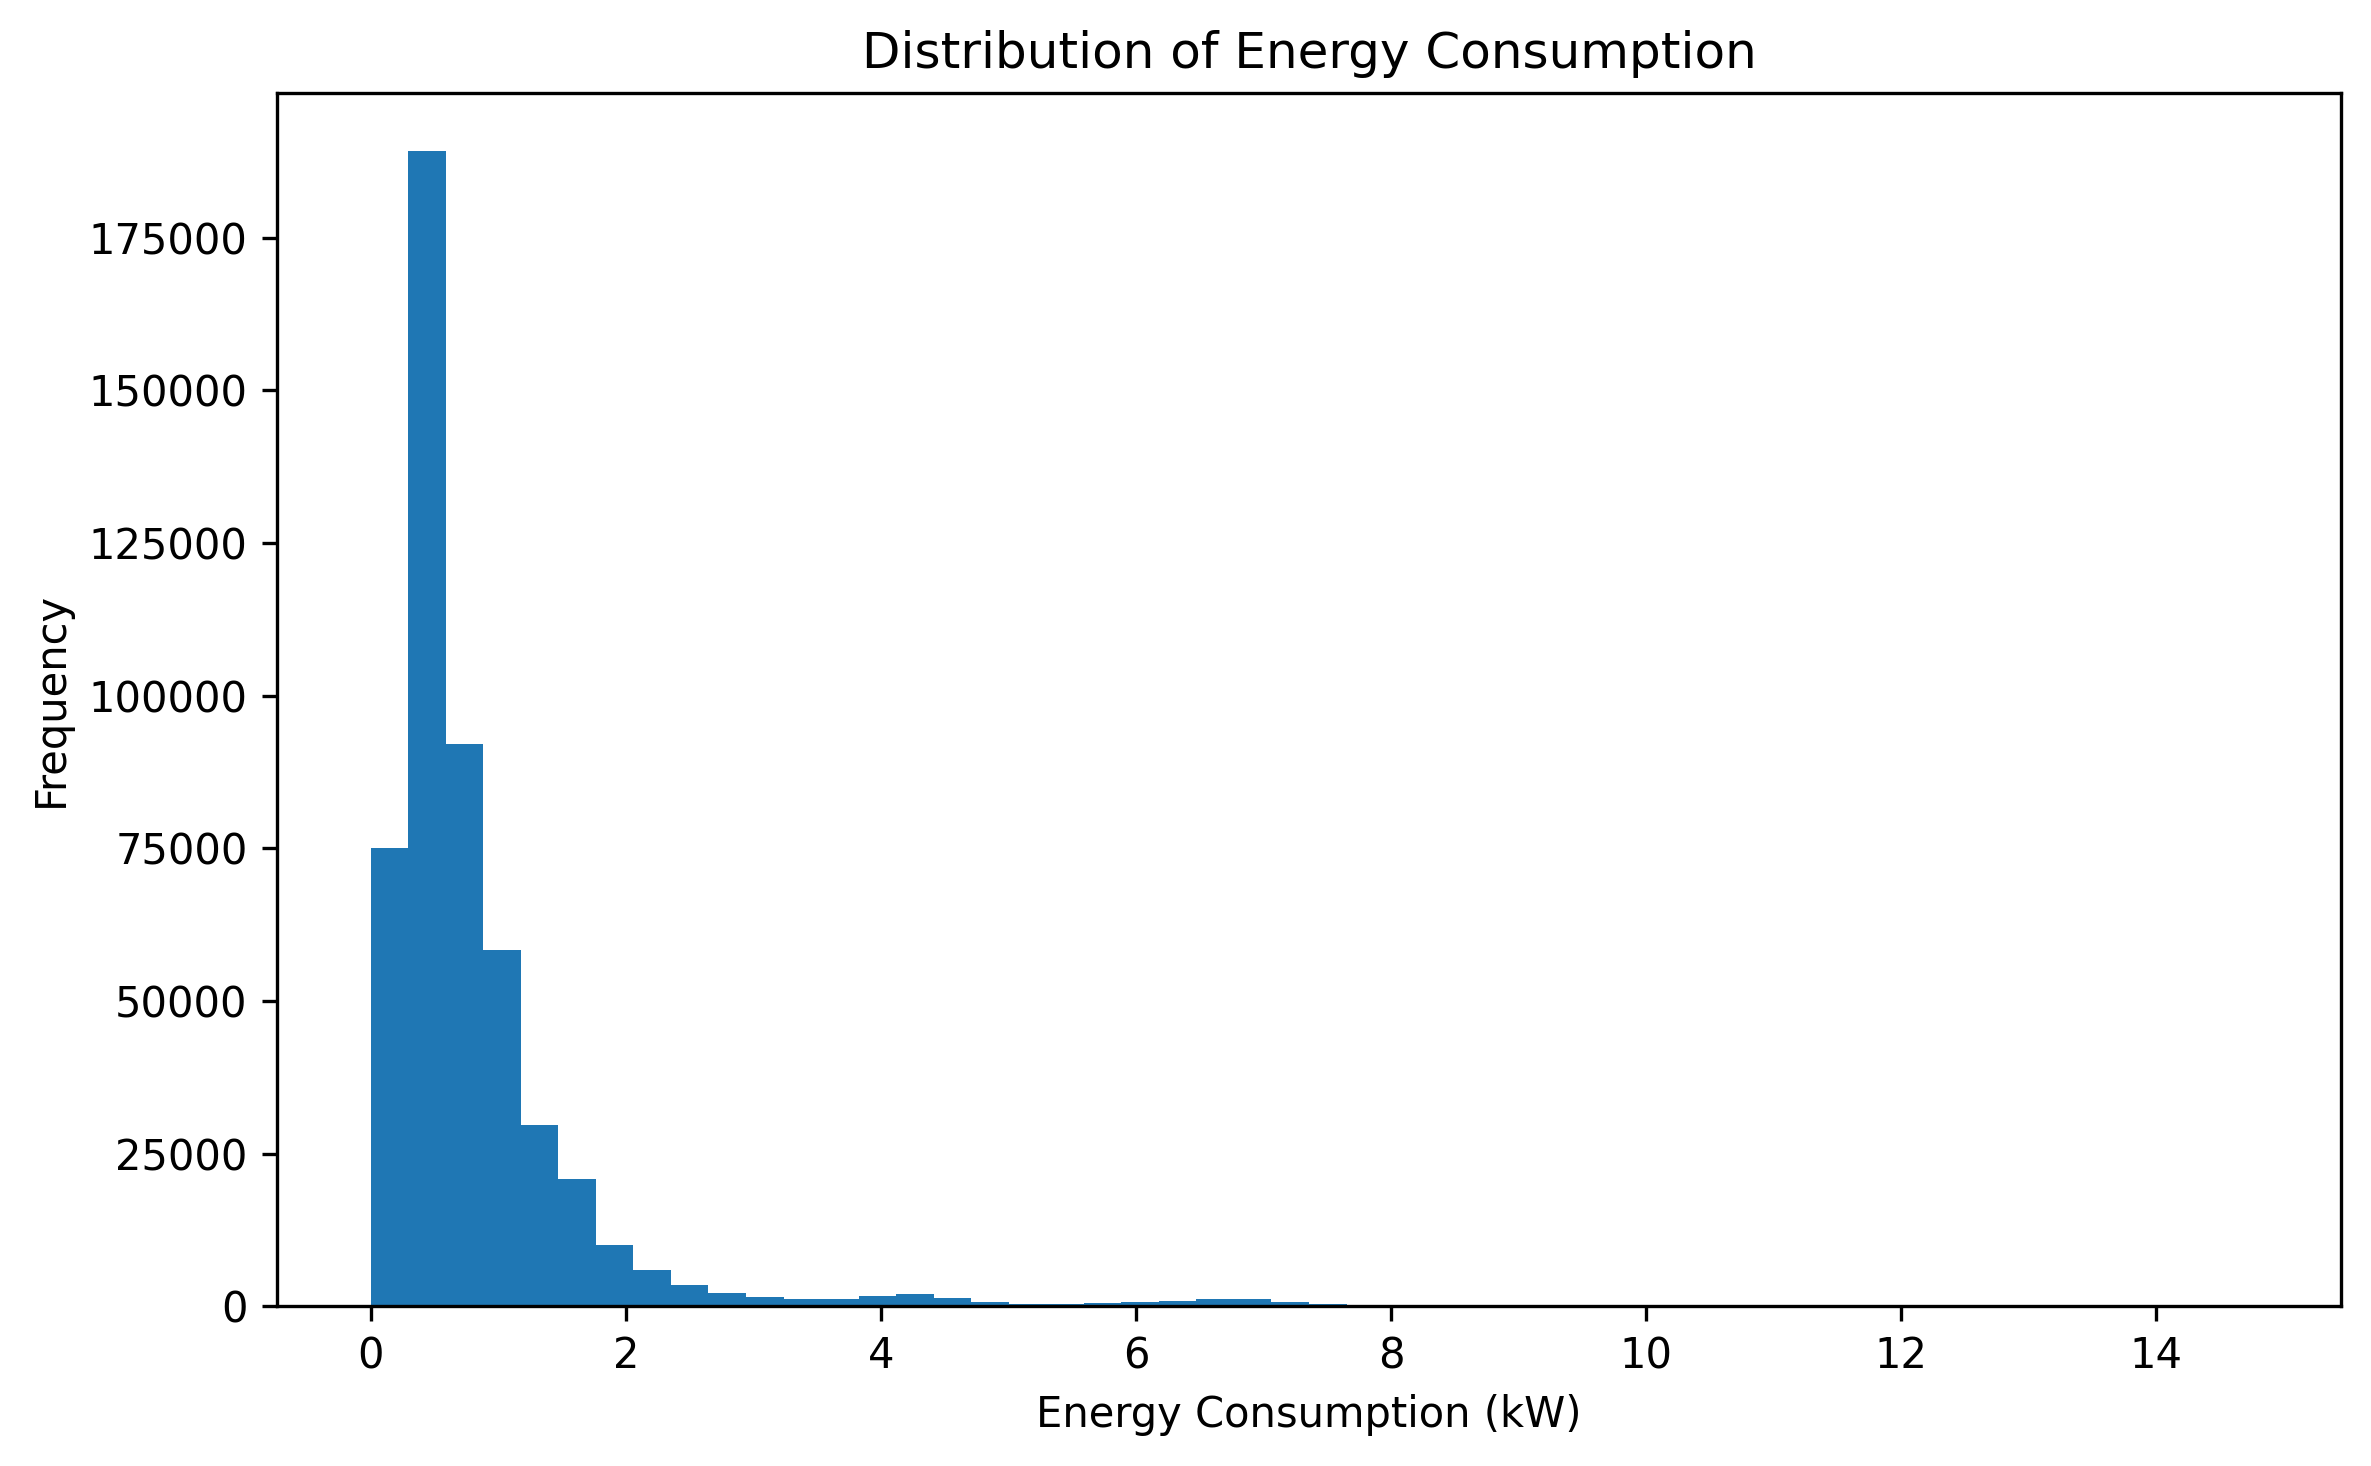
\includegraphics[width=0.7\textwidth]{chart2_histogram.png}
\caption{Distribution of total energy consumption. The distribution is strongly right-skewed: most observations occur at low consumption levels, while high-consumption events are comparatively rare.}\label{fig:hist}
\end{figure}

The right-skewed distribution in Figure~\ref{fig:hist} confirms that high-consumption events are infrequent, supporting the rare-event framing and the choice of imbalance-aware metrics.

\begin{figure}[h]
\centering
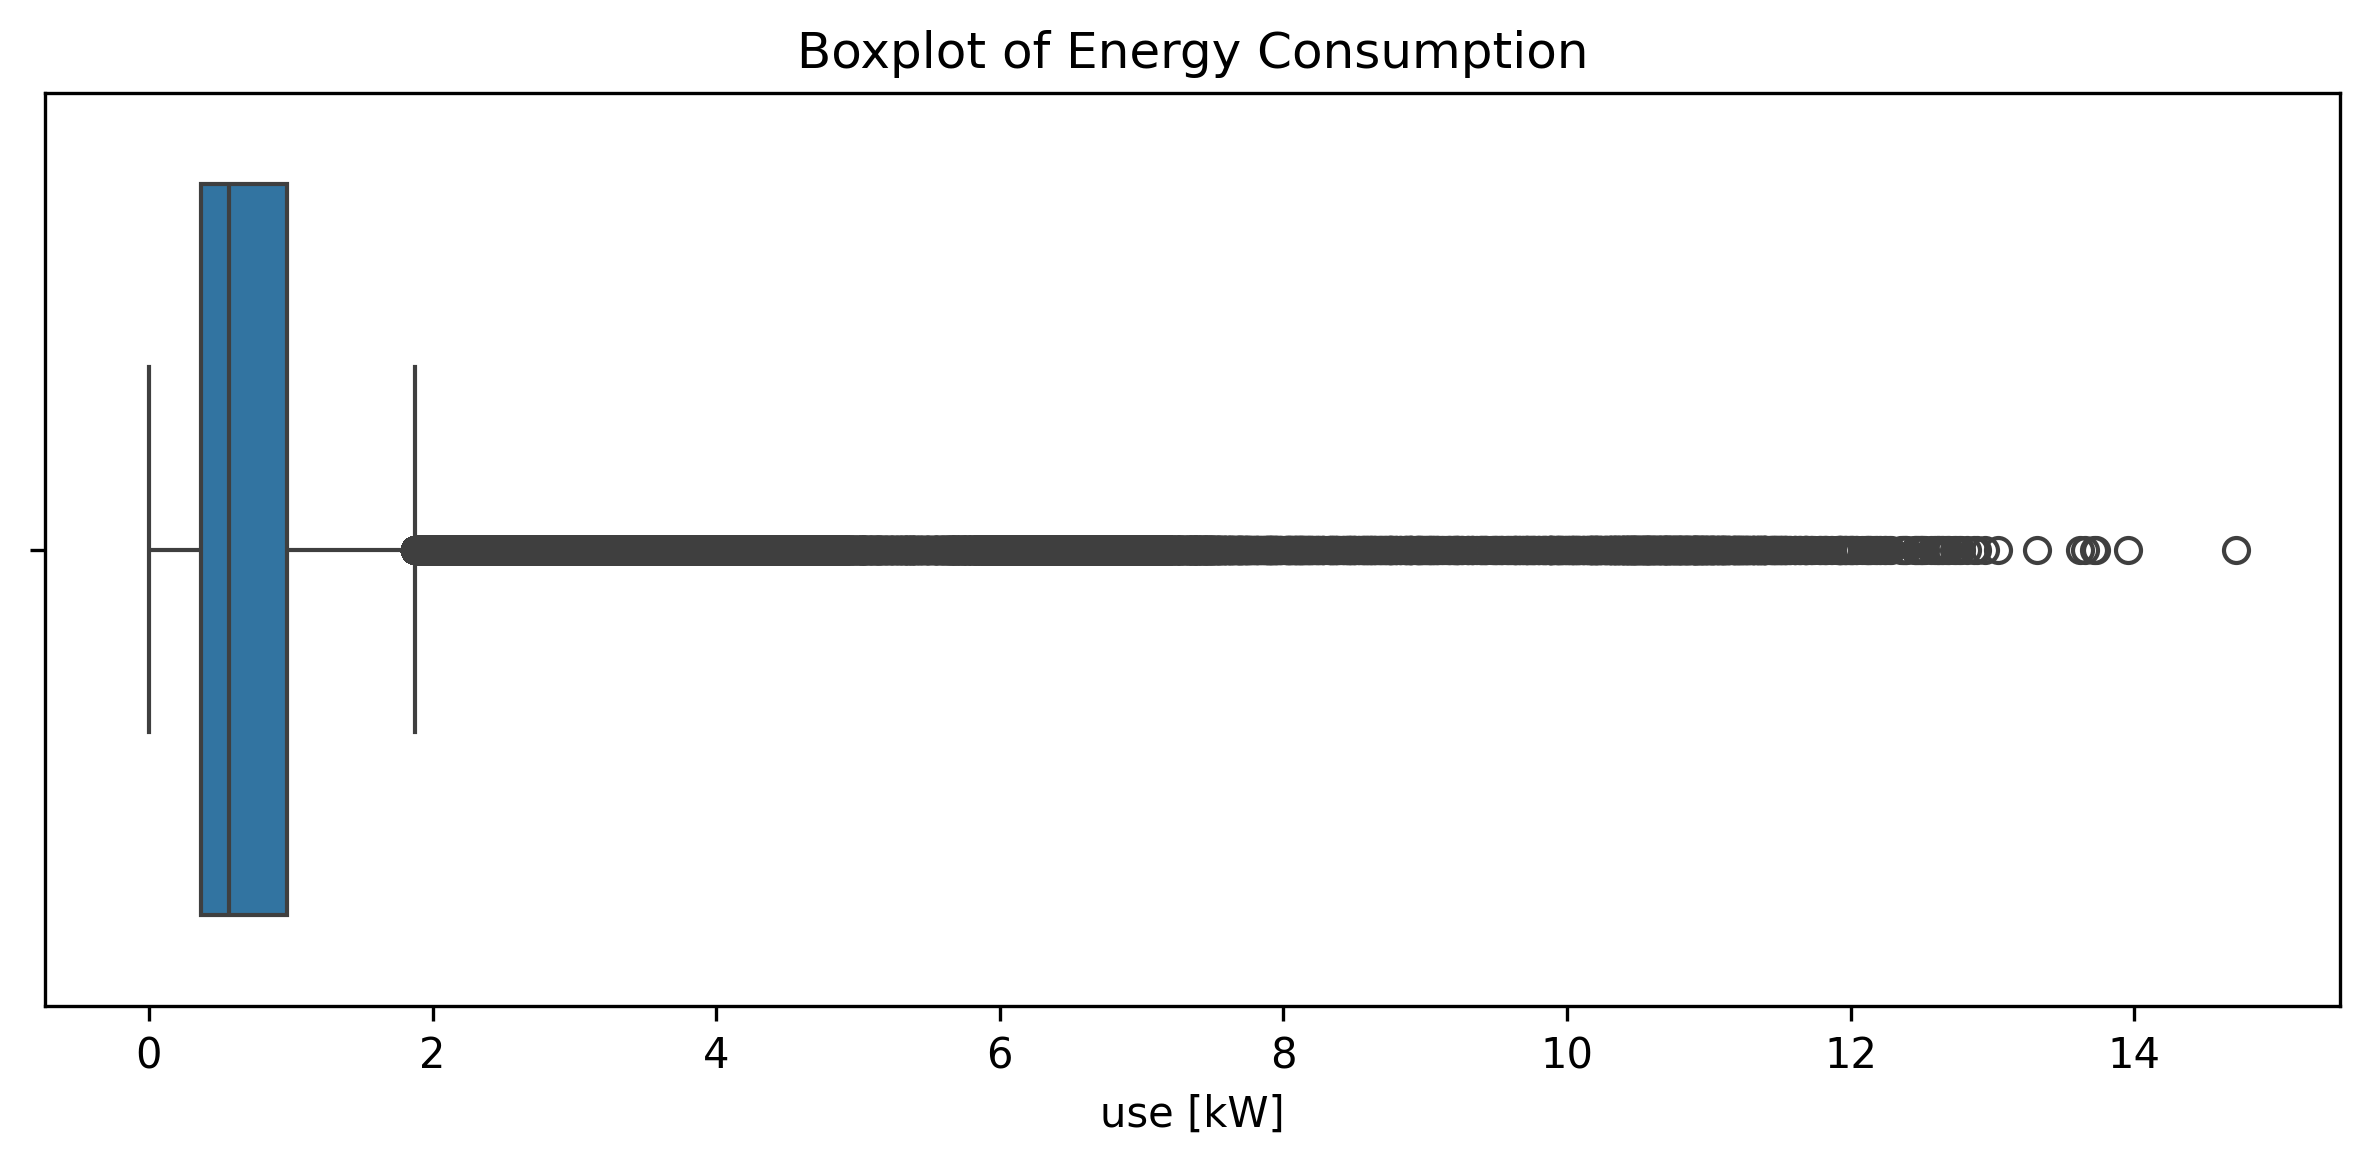
\includegraphics[width=0.7\textwidth]{chart3_boxplot.png}
\caption{Boxplot of total energy consumption. Numerous observations beyond the whiskers indicate extreme values and potential outliers.}\label{fig:box}
\end{figure}

Figure~\ref{fig:box} reinforces the presence of many extreme values, consistent with the IQR-based outlier count reported in Section~\ref{subsec:clean}.

\begin{figure}[h]
\centering
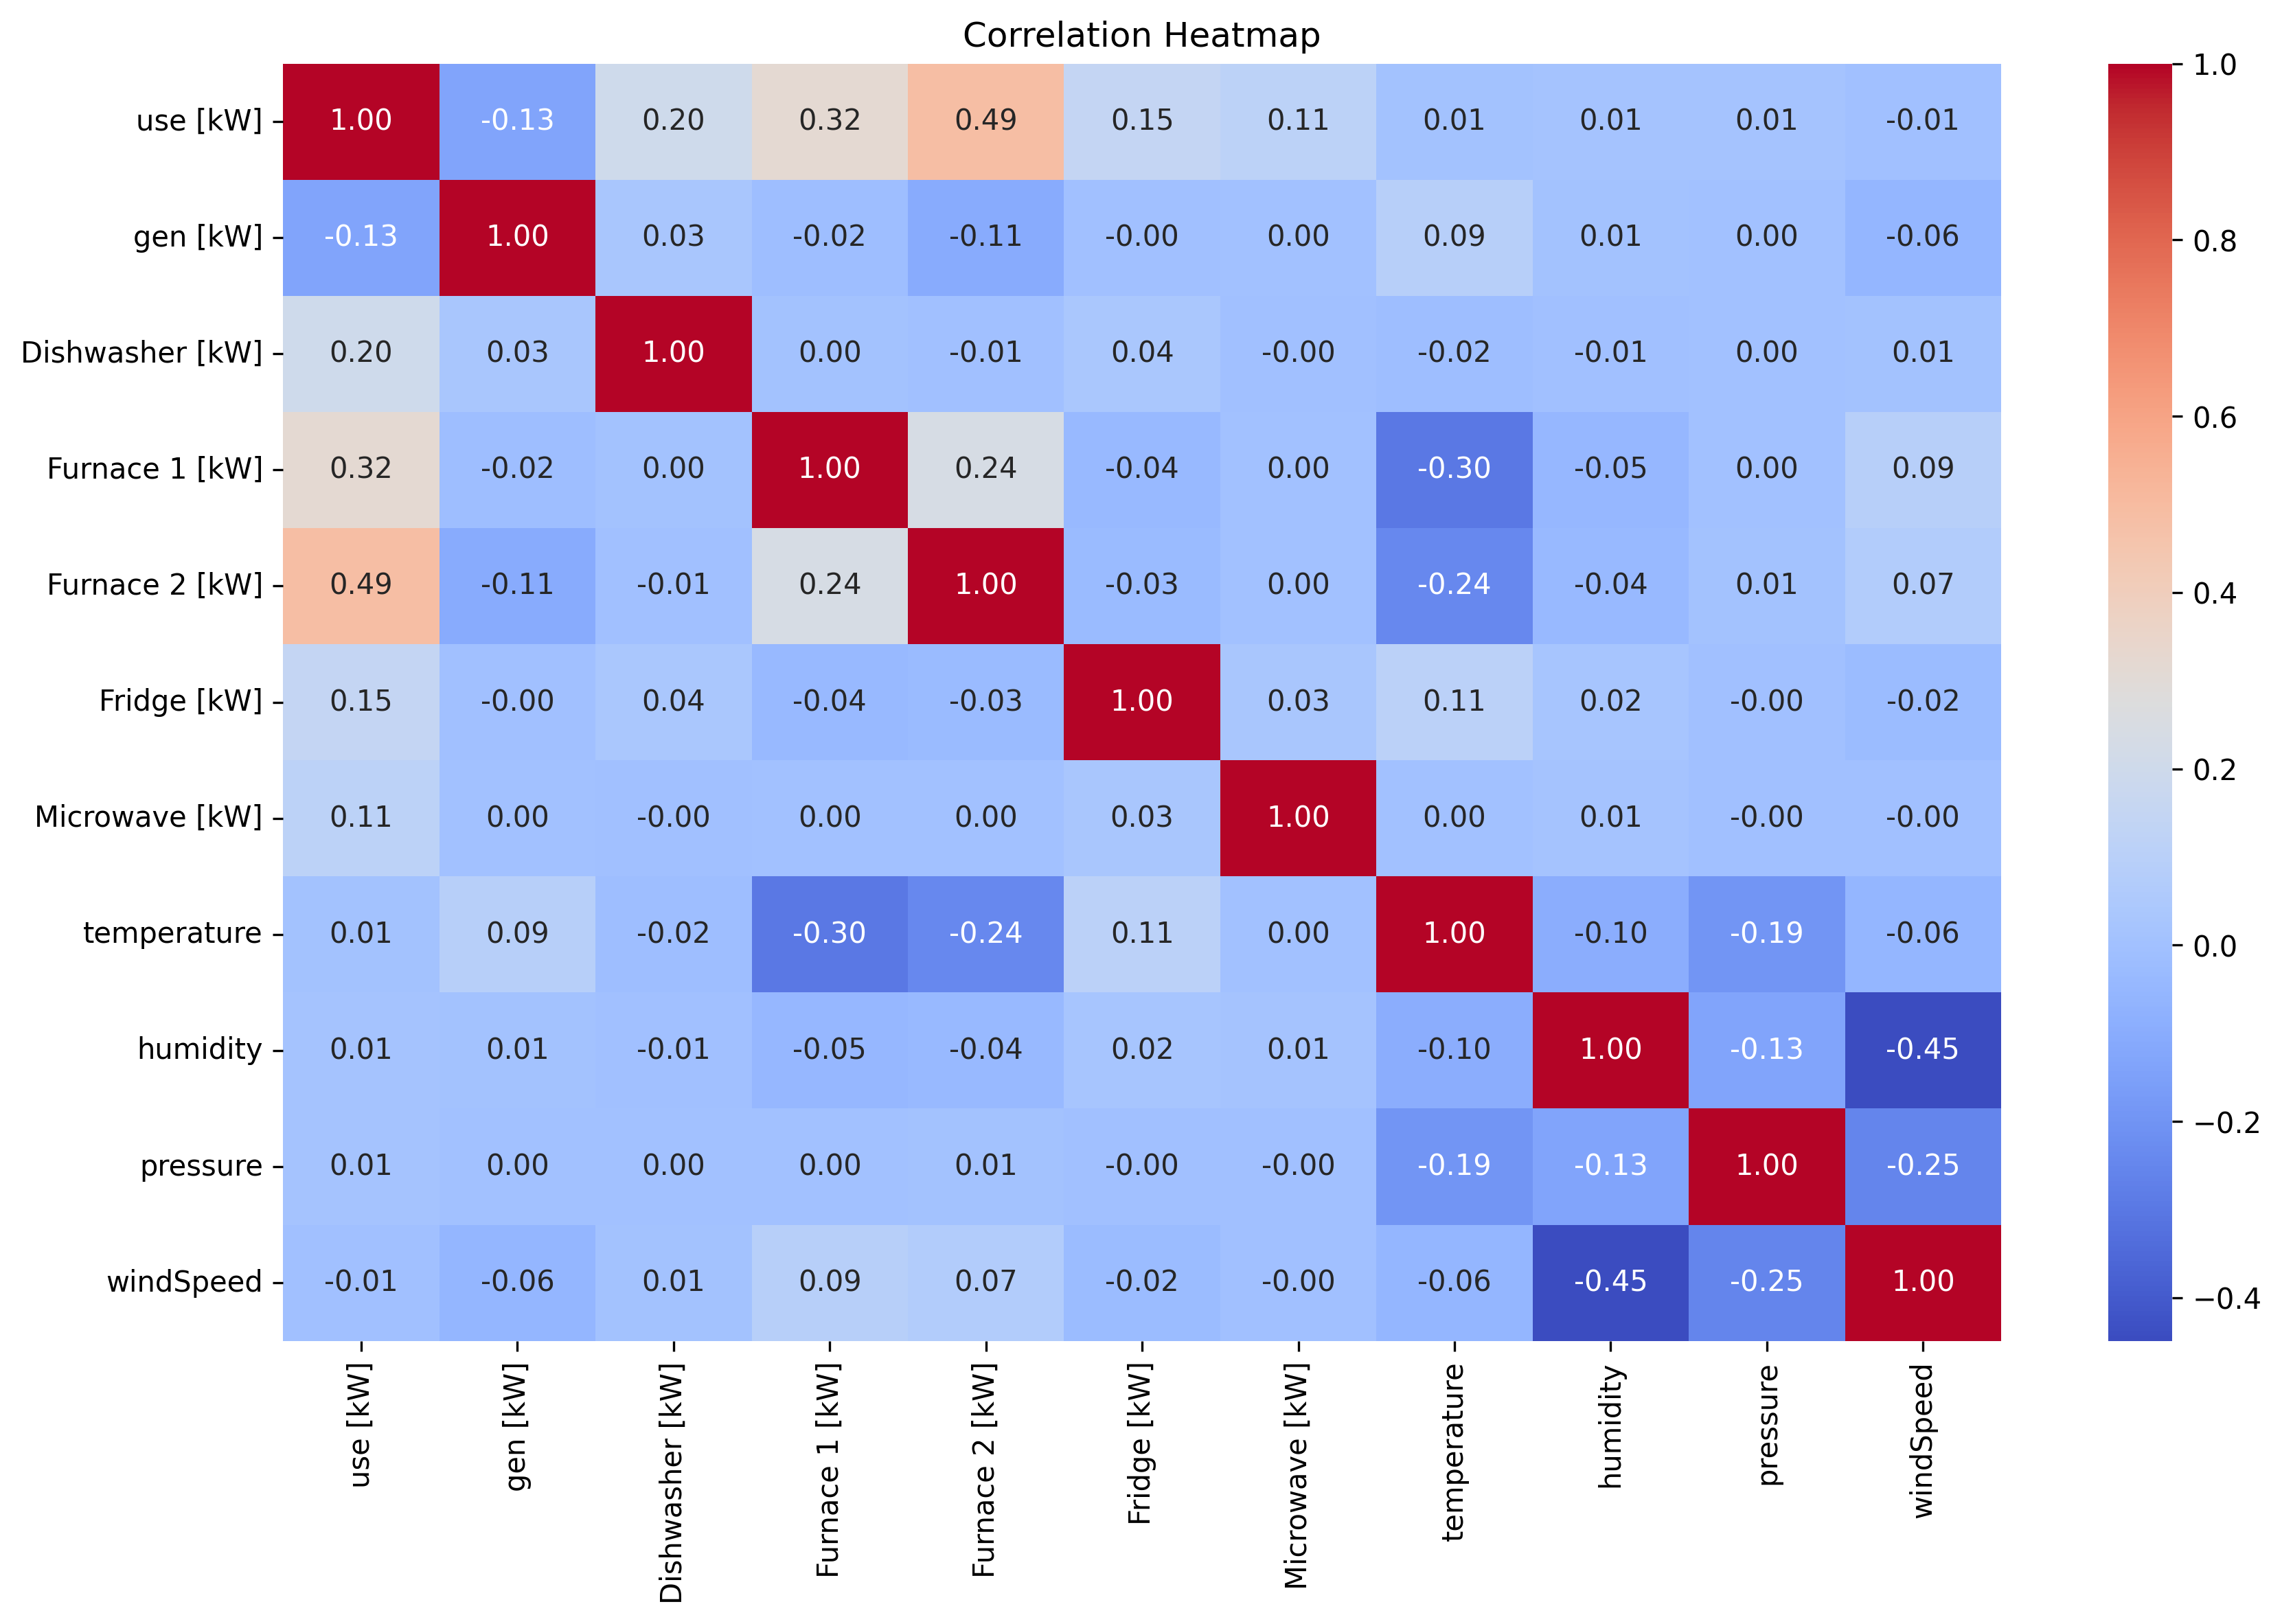
\includegraphics[width=0.95\textwidth]{chart4_heatmap.png}
\caption{Correlation heatmap among energy, appliance and weather variables. Several appliance variables show moderate-to-strong correlation with total consumption, while weather variables show weaker relationships.}\label{fig:heat}
\end{figure}

Figure~\ref{fig:heat} indicates that appliance-level variables are more strongly correlated with total consumption than weather variables, which partly addresses RQ1 and RQ3: appliance load appears to be the dominant driver, with weather contributing a weaker signal.

%%=============================================================%%
\section{Results}\label{sec6}

Table~\ref{tab:results} reports the performance of all five models on the held-out test partition.

\begin{table}[h]
\caption{Model comparison on the held-out test set. Best F1 in bold.}\label{tab:results}%
\begin{tabular}{@{}lcccc@{}}
\toprule
Model & F1 & AUC & Precision & Recall\\
\midrule
Random Forest        & \textbf{0.9343} & 0.9995 & 0.9164 & 0.9529 \\
XGBoost              & 0.9308 & 0.9994 & 0.9145 & 0.9477 \\
LightGBM             & 0.8855 & 0.9986 & 0.8285 & 0.9509 \\
Logistic Regression  & 0.3686 & 0.9683 & 0.2301 & 0.9267 \\
Isolation Forest     & 0.0818 & 0.7464 & 0.0831 & 0.0805 \\
\botrule
\end{tabular}
\footnotetext{Metrics computed against the statistical proxy label of Eq.~\eqref{eq:label}, not externally validated ground truth.}
\end{table}

Addressing RQ2, Random Forest achieved the highest F1-score (0.9343) and AUC (0.9995), narrowly ahead of XGBoost. The tree-ensemble models clearly outperformed Logistic Regression, whose low precision (0.2301) indicates many false positives despite high recall. The unsupervised Isolation Forest performed markedly worse than the supervised models (F1 = 0.0818, AUC = 0.7464).

This large gap between the supervised models and Isolation Forest is informative but must be interpreted carefully. The supervised models are trained and evaluated against the same statistical proxy definition, so part of their advantage reflects their ability to recover the threshold rule that generated the labels, rather than the discovery of independently validated anomalies. Isolation Forest, by contrast, identifies structural outliers without access to that rule. The contrast therefore illustrates the difference between the two paradigms under proxy supervision rather than establishing the superiority of supervised methods for true anomaly detection.

%%=============================================================%%
\section{Deployment}\label{sec7}

The final pipeline, comprising standardisation and the selected model, was serialised together with the ordered list of 55 feature columns to ensure that inference uses the same feature ordering as training. The pipeline was integrated into an interactive dashboard that accepts a single observation, constructs the full feature vector (with unspecified inputs defaulting to zero), and returns a normal/abnormal prediction. An optional natural-language explanation component is available, with a rule-based fallback when no external service is configured.

%%=============================================================%%
\section{Discussion and Limitations}\label{sec8}

Three limitations qualify the findings. First, and most importantly, the labels are a statistical \emph{proxy}; the reported metrics measure agreement with Eq.~\eqref{eq:label} rather than detection of verified anomalies, and the high supervised scores partly reflect recovery of the labelling rule. Second, the dataset's timestamp issue restricts the validity of seasonal temporal features, so conclusions about monthly or weekly seasonality should be treated as inconclusive. Third, the comparison excludes kernel SVM models for scalability reasons, so the model space is not exhaustive.

Despite these constraints, the study provides a transparent, reproducible pipeline and a clear like-for-like comparison of model families on the same partition. The honest framing of the proxy label is itself a contribution: it makes explicit an assumption that is frequently left implicit in applied energy-anomaly work \cite{ambat2025}.

%%=============================================================%%
\section{Conclusion}\label{sec9}

We presented an anomaly-detection study on the HomeC smart home energy dataset, reformulating an unlabelled time-series problem as binary classification through a transparent statistical proxy label. Among five models, Random Forest performed best against the proxy definition (F1 = 0.9343, AUC = 0.9995), while the unsupervised Isolation Forest performed substantially worse, highlighting the role of proxy supervision. Exploratory analysis suggested that appliance-level variables are more strongly associated with abnormal consumption than weather variables (RQ1, RQ3). Future work should pursue externally validated anomaly labels, address the dataset's timestamp limitation at source, and incorporate contextual or knowledge-driven explanations to move beyond purely statistical proxies.

%%=============================================================%%
\backmatter

\bmhead{Acknowledgements}
The authors thank the course instructor for guidance, and acknowledge the use of AI assistance for code drafting and editing, with all design decisions, verification and final analysis performed by the authors.

\section*{Declarations}

\begin{itemize}
\item \textbf{Data availability:} The Smart Home Dataset with Weather Information (HomeC) is publicly available on Kaggle.
\item \textbf{Competing interests:} The authors declare no competing interests.
\item \textbf{Code availability:} Source code and the trained pipeline are maintained in the project repository.
\end{itemize}

\bibliography{references}

\end{document}
